\documentclass[tikz,border=8pt]{standalone}
\usepackage{fontspec}\setsansfont{Noto Sans}
\usetikzlibrary{arrows.meta,positioning,calc}
\definecolor{Ink}{HTML}{182B3A}
\definecolor{Blue}{HTML}{145AAD}
\definecolor{Purple}{HTML}{703F91}
\definecolor{Teal}{HTML}{007367}
\begin{document}
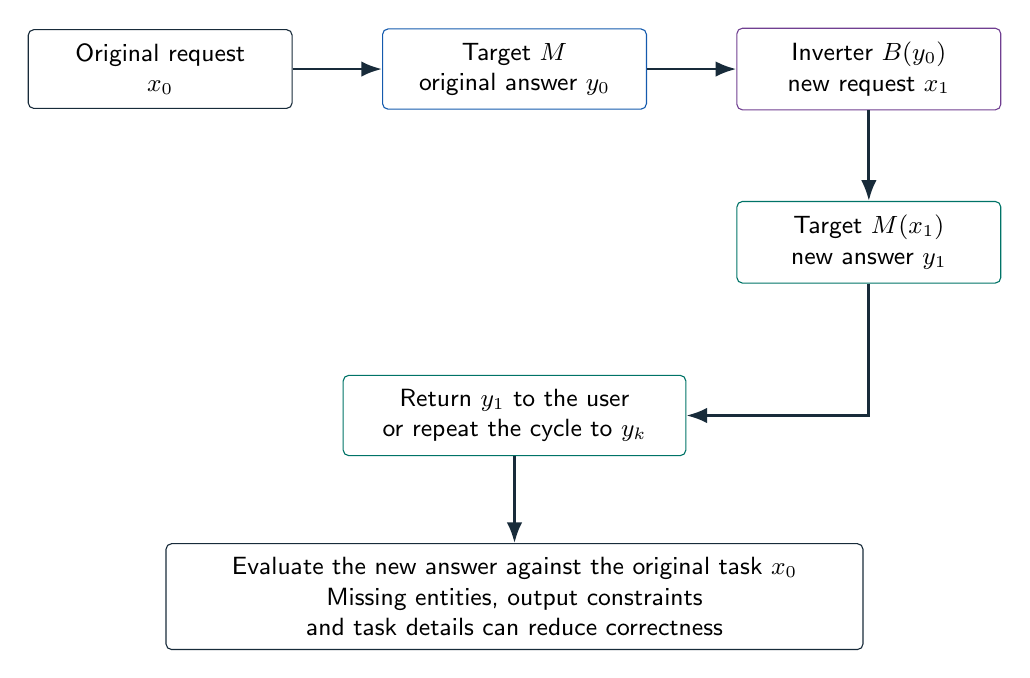
\begin{tikzpicture}[font=\sffamily\small,>=Latex,box/.style={draw=Ink,rounded corners=2pt,align=center,text width=3.0cm,minimum height=1cm,inner sep=5pt},flow/.style={->,line width=1pt,draw=Ink}]
 \node[box] (x) at (0,0) {Original request\\\(x_0\)};
 \node[box,draw=Blue] (y) at (4.5,0) {Target \(M\)\\original answer \(y_0\)};
 \node[box,draw=Purple] (b) at (9,0) {Inverter \(B(y_0)\)\\new request \(x_1\)};
 \node[box,draw=Teal] (forward) at (9,-2.2) {Target \(M(x_1)\)\\new answer \(y_1\)};
 \node[box,text width=4.0cm,draw=Teal] (return) at (4.5,-4.4) {Return \(y_1\) to the user\\or repeat the cycle to \(y_k\)};
 \node[box,text width=8.5cm] (eval) at (4.5,-6.7) {Evaluate the new answer against the original task \(x_0\)\\Missing entities, output constraints and task details can reduce correctness};
 \draw[flow] (x)--(y); \draw[flow] (y)--(b);
 \draw[flow] (b)--(forward);
 \draw[flow] (forward.south) |- (return.east);
 \draw[flow] (return)--(eval);
\end{tikzpicture}
\end{document}
